\section{Twierdzenie Andersona-Schoriego o spłaszczaniu rozmaitości}

\begin{lem} \label{lem:flat}
  Niech $X$ będzie przestrzenią metryczną z RIP, a $Y = X^{\mathbb{N}_1}$. Niech $V$ będzie zbiorem otwartym w $Y$ i $A, B \subset V$ takie, że $B = \cl{B}$ oraz $A = \cl{A} \cap V$. Oznaczmy przez $p$ projekcję z definicji zredukowanego produktu $(V \times X)_A$. Wówczas istnieje zbiór $C$: $B \subset C = \cl{C} \subset V$ i homeomorfizm $h$ zbioru $(V \times X)_A$ na $(V \times X)_{A \cup B}$ o następującej własności:
  
  \begin{equation} \label{eq:as-lem-1}
  h(z) = z \mbox{ dla } p(z) \in (V \setminus C) \cup A
  \end{equation}
  \begin{proof}
    Niech
    \[L := \{y \in Y\ |\ d(y, Y \setminus V) \leq d(y, B)\}\]
    
    Do dowodu będziemy potrzebować funkcji sterujących $\lambda$ i $\rho$ o następujących własnościach:
    \begin{gather}
      \label{lambda-infty} \lambda(y) = \infty \Leftrightarrow y \in (Y \setminus V) \cup A \cup B \\
      \label{rho-infty} \rho(y) = \infty \Leftrightarrow y \in (Y \setminus V) \cup A \\
      \label{rho-eq-lambda} \rho(y) = \lambda(y), \mbox{ dla } y \in A \cup L \\
      \label{rho-dist} 2^{-\rho(y)} \leq \frac{1}{4} d(y, Y \setminus V)
    \end{gather}
    
    Konstrukcja:
    Zauważmy, że $(Y \setminus V) \cup A = (Y \setminus V) \cup (\cl{A} \cap V) = (Y \setminus V) \cup \cl{A}$, więc $(Y \setminus V) \cup A$ jest zbiorem domkniętym. Podobnie $A \cup L$ jest zbiorem domkniętym, gdyż $Y \setminus V \subset L$.
    
    Niech $\lambda_0$ będzie funkcją sterującą z wniosku \ref{cor:steering-finite} dla zbioru domkniętego $(Y \setminus V) \cup A \cup B$. Przez $\rho_0$ oznaczmy funkcję sterującą $\lambda_0$ poprawioną (twierdzenie \ref{thm:steering-function}) na zbiorze domkniętym $A \cup L$.
    
    \begin{figure}[h!]
      \centering
      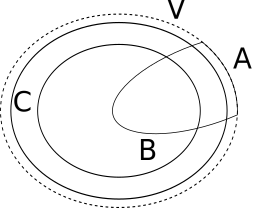
\includegraphics[scale=.5]{img/first-flatten.pdf}
      \caption{Sytuacja z lematu \ref{lem:flat}}
    \end{figure}
    
    Skoro $\rho_0(y)$ poza $A \cup L$ jest skończone a na $A \cup L$ jest równe $\lambda_0$, to $\rho_0(y) = \infty$ wtedy i tylko wtedy gdy $y \in (A \cup L) \cap ((Y \setminus V) \cup A \cup B) = (Y \setminus V) \cup A$
    
    Otrzymaliśmy więc funkcje następujące:
    \begin{gather}
      \lambda_0(y) = \infty \Leftrightarrow y \in (Y \setminus V) \cup A \cup B \\
      \rho_0(y) = \infty \Leftrightarrow y \in (Y \setminus V) \cup A \\
      \label{rho0-eq-lambda0} \rho_0(y) = \lambda_0(y) \mbox{ dla } y \in A \cup L
    \end{gather}
    
    Dalej weźmy funkcję sterującą $\mu$ z wniosku \ref{cor:steering-dist} dla zbioru domkniętego $Y \setminus V$. Mamy więc:
    \begin{gather}
      \mu(y) = \infty \Leftrightarrow y \in Y \setminus V \\
      2^{-\mu(y)} \leq \frac{1}{4} d(y, Y \setminus V)
    \end{gather}
    
    Po tych przygotowaniach połóżmy:
    \begin{gather*}
      \lambda := \max(\lambda_0, \mu) \\
      \rho := \max(\rho_0, \mu)
    \end{gather*}
    Z własości funkcji sterujących wiemy, że $\lambda$ i $\rho$ są również funkcjami sterującymi.
    
    Wykażemy, że spełnione są postulowane warunki:
    \begin{align*}
     \lambda(y) = \infty & \Leftrightarrow \max(\lambda_0, \mu)(y) = \infty \\
     & \Leftrightarrow \lambda_0(y) = \infty \vee \mu(y) = \infty \\
     & \Leftrightarrow y \in ((Y \setminus V) \cup A \cup B) \cup (Y \setminus V) \\
     & \Leftrightarrow y \in (Y \setminus V) \cup A \cup B
    \end{align*}
    a więc zachodzi warunek \eqref{lambda-infty}.
    
    Dalej:
    \begin{align*}
      \rho(y) = \infty & \Leftrightarrow \max(\rho_0, \mu)(y) = \infty \\
      & \Leftrightarrow \rho_0(y) = \infty \vee \mu(y) = \infty \\
      & \Leftrightarrow y \in ((Y \setminus V) \cup A) \cup (Y \setminus V) \\
      & \Leftrightarrow y \in (Y \setminus V) \cup A
    \end{align*}
    więc spełniony jest warunek \eqref{rho-infty}
    
    Skoro z \eqref{rho0-eq-lambda0} wynika, że funkcje $\lambda_0$ i $\rho_0$ na $A \cup L$ są sobie równe, to po wzięciu maksimum z $\mu$ warunek ten zostanie zachowany, co daje nam \eqref{rho-eq-lambda}.
    
    Pozostaje jeszcze \eqref{rho-dist}, które wynika z nierówności:
    \[2^{-\rho(y)} \leq 2^{-\mu(y)} \leq \frac{1}{4} d(y, Y \setminus V)\]
    
    Z twierdzenia o istnieniu homotopii spychającej \ref{thm:displacement-homotopy} możemy wziąć $(f_t)_{1 \leq t \leq \infty}$ homotopię spychającą.
    Z wniosku pierwszego twierdzenia o spłaszczaniu istnieje homeomorfizm:
    
    \[g: (Y \times X)_{(Y \setminus V) \cup A \cup B} \rightarrow Y\]
    
    generowany przez funkcję sterującą $\lambda$ i homotopię $(f_t)_{1 \leq t \leq \infty}$, identycznościowy nad $(Y \setminus V) \cup A \cup B$ oraz:
    
    \[f: (Y \times X)_{(Y \setminus V) \cup A} \rightarrow Y\]
    
    generowany przez funkcję sterującą $\rho$ i homotopię $(f_t)_{1 \leq t \leq \infty}$, identycznościowy nad $(Y \setminus V) \cup A$. Oba te homeomorfizmy są więc w szczególności identycznościowe nad $Y \setminus V$. Z uwagi na lemat \ref{lem:reduced-product-subspace} podprzestrzeń $(V\times X)_{A\cup B}$ przestrzeni $(Y\times X)_{(Y\setminus V)\cup A\cup B}$ możemy traktować zarówno jako podprzestrzeń z topologią indukowaną jak i podprzestrzeń z topologią zredukowanego produktu. Podobnie podprzestrzeń $(V\times X)_{A}$ przestrzeni $(Y\times X)_{(Y\setminus V)\cup A}$ jest taka sama z topologią zredukowanego produktu jak i topologią indukowaną z $(Y\times X)_{(Y\setminus V)\cup A}$. Zatem następujące odwzorowania są homeomorfizmami:
    \begin{itemize}
     \item $g|(V \times X)_{A \cup B}: (V \times X)_{A \cup B} \to V$
     \item $f|(V \times X)_{A}: (V \times X)_{A} \to V$
    \end{itemize}

    Oznaczmy te zawężenia odpowiednio przez $g$ i $f$.
    
    Definiujemy żądany homeomorfizm jako:
    \[h := g^{-1} f: (Y \times X)_{A} \rightarrow (Y \times X)_{A \cup B}\]
    
    Należy jeszcze znaleźć $C$, dla którego zachodzi warunek \eqref{eq:as-lem-1}. Zdefiniujmy:
    \[C := \{y \in Y\ |\ d(y,B) \leq 4 d(y, Y \setminus V)\}\]
    
    Jeśli $p(z) \in A$, to $p(z) = z$ oraz $f(z) = z$ i $g(z) = z$, więc $h(z) = g^{-1}(f(z)) = g^{-1}(z) = z$. Niech teraz $p(z) \in V \setminus C$. Wówczas z definicji zbioru $C$ mamy:
    
    \begin{equation}
      \label{dist-pz-YV} d(pz, Y \setminus V) \leq \frac{1}{4} d(pz, B)
    \end{equation}
    
    Wykażemy teraz, że:
    \begin{equation}
      \label{dist-fz-pz-0}d(fz, pz) \leq 2^{-\rho(pz)} \cdot 2
    \end{equation}
    
    Jeśli $pz \in A$, to $\rho(pz) = \infty$, więc $fz = f_{\rho(pz)}(z) = pz$. A zatem $d(fz, pz) = 0$.
    
    W przeciwnym razie $fz = f_{\rho(pz)}(z)$, a więc z własności homotopii spychającej dla $k \leq \rho(pz)$ mamy:
    
    \[s_k fz = s_k pz\]
    
    Zatem $d(fz, pz) \leq 2^{-\rho(pz)} \cdot 2$.
    
    Z nierówności \eqref{dist-fz-pz-0} i \eqref{rho-dist} otrzymujemy:
    \begin{equation}
      \label{dist-fz-pz} d(fz, pz) \leq \frac{1}{2} d(pz, Y \setminus V)
    \end{equation}
    
    Mamy także:
    \begin{equation}
      \label{dist-pz-fz-B} d(pz, fz) \overset{\eqref{dist-fz-pz}}{\leq} \frac{1}{2} d(pz, Y \setminus V) \overset{\eqref{dist-pz-YV}}{\leq} \frac{1}{8} d(pz, B)
    \end{equation}


    Następnie przyjrzyjmy się nierównościom:
    \begin{align*}
      d(fz, Y \setminus V) & \leq d(fz, pz) + d(pz, Y \setminus V) \\
      & \leq \frac{1}{2} d(pz, Y \setminus V) + d(pz, Y \setminus V) = \frac{3}{2} d(pz, Y \setminus V) & \mbox{z \eqref{dist-fz-pz}} \\
      & \leq \frac{3}{2} \cdot \frac{1}{4} d(pz, B) & \mbox{z \eqref{dist-pz-YV}} \\
      & \leq \frac{7}{8} d(pz, B) = d(pz, B) - \frac{1}{8} d(pz, B) \\
      & \leq d(pz, B) - d(pz, fz) & \mbox{z \eqref{dist-pz-fz-B}} \\
      & \leq d(fz, B)
    \end{align*}
    
    Z powyższej nierówności wnioskujemy, że $fz \in L$. Ale wówczas z \eqref{rho-eq-lambda} otrzymujemy $\lambda(fz) = \rho(fz)$. Ale wówczas otrzymujemy:
    \[hz = g^{-1}fz = f^{-1}_{\lambda(fz)}(fz) = f^{-1}_{\rho(fz)}(f_{\rho(fz)}(z)) = z\]
  \end{proof}

\end{lem}

\begin{lem} \label{lem:manifold-homeo}
  Niech $M$ będzie $Y$-rozmaitością, gdzie $Y$ jest przestrzenią liniowo-metryczną taką, że $Y$ jest homeomorficzne z $Y^\Ni$. Niech $f: U \to V$ będzie mapą regularną na $M$. Weźmy $A_1$, $A_2$ domknięte podzbiory $M$, gdzie $A_2 \subset U$. Wówczas istnieje homeomorfizm $g: (M\times Y)_{A_1} \to (M\times Y)_{A_1 \cup A_2}$ taki, że $g(z) = z\ \forall pz \in (M\setminus U) \cup A_1$.
  
  \begin{proof}
    Niech $A := \cl{f}(A_1 \cap U)$, $B := \cl{f}(A_2)$, $X := Y$. Skoro $A_2$ domknięty w $M$, to jest też domknięty w $\cl U$, skąd $B$ domknięty w $\cl{f}(\cl U)$, a więc z regularności mapy $f$ i w $Y$. Skoro $A_1 \cap U$ domknięty w $U$, to $\cl{f}(A_1 \cap U) = f(A_1 \cap U) = A$ domknięty w $V$.
    
    \begin{figure}[h!]
      \centering
      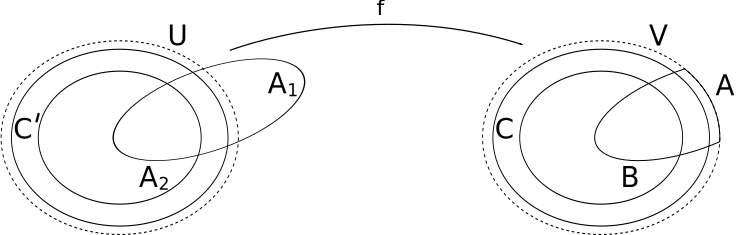
\includegraphics[scale=.5]{img/lem-homeo.pdf}
      \caption{Sytuacja z lematu \ref{lem:manifold-homeo}}
    \end{figure}
    
    Co więcej, $X$ jako produkt przestrzeni $Y$ jest homeomorficzny z $X^2$ (oraz z $X^\Ni$) więc z wniosku \ref{cor:rip-space} $X$ jest przestrzenią z RIP. Na mocy lematu \ref{lem:flat} otrzymujemy homeomorfizm
    \[
      h: (V\times Y)_{A} \to (V\times Y)_{A\cup B},
    \]
    który nad $(V\setminus C)\cup A$ jest identycznościowy, gdzie $C$ jest pewnym domkniętym nadzbiorem $B$ zawartym w $V$, tzn. $B \subset C = \cl C \subset V$. Niech $C' := \cl{f}^{-1}(C)$ będzie domkniętym nadzbiorem $A_2$ zawartym w $U$.
    Weźmy homeomorfizmy:
    \[
      F_1: (U\times Y)_{A_1 \cap U} \to (V\times Y)_A
    \]
    oraz
    \[
      F_2: (U\times Y)_{(A_1 \cap U)\cup A_2} \to (V\times Y)_{A\cup B}
    \]
    wygenerowane z lematu \ref{lem:reduced-product-homeo} przez homeomorfizm $f: U\to V$.

    Otrzymujemy homeomorfizm między zbiorami otwartymi:
    \[
      g' := F_2^{-1} \circ h \circ F_1: (U\times Y)_{A_1 \cap U} \to (U\times Y)_{(A_1\cap U) \cup A_2}
    \]
    Ze względu na lemat \ref{lem:reduced-product-subspace} przestrzeń $(U\times Y)_{A_1 \cap U}$ traktujemy jako podprzestrzeń $(M\times Y)_{A_1}$. Podobnie przestrzeń $(U\times Y)_{(A_1\cap U)\cup A_2}$ traktujemy jako podrzestrzeń $(M\times Y)_{A_1\cup A_2}$.
    Weźmy odwzorowanie identycznościowe:
    \[
      g'' := \id: ((M\setminus C')\times Y)_{A_1\setminus C'} \to ((M\setminus C')\times Y)_{A_1\setminus C'}.
    \]
    Znowu ze względu na lemat \ref{lem:reduced-product-subspace} przsetrzeń $((M\setminus C')\times Y)_{A_1\setminus C'}$ traktujemy jako podzbiór w przestrzeni $(M\times Y)_{A_1}$ w dziedzinie oraz jako podzbiór przestrzeni $(M\times Y)_{A_1\cup A_2}$ w obrazie. Co więcej, jest on podzbiorem otwartym każdej z tych przestrzeni.
    
    Zauważmy, że $g'$ i $g''$ można skleić do homeomorfizmu $g$, ponieważ na zbiorze otwartym $\dom g'\cap \dom g'' = ((U\setminus C')\times Y)_{A_1 \cap (U\setminus C')}$ odwzorowanie $g'$ jest idetycznościowe. Istotnie, weźmy takie $z$. Wówczas $F_1(z) \in ((V\setminus C) \times Y)_{A}$, a więc $h$ działa na ten punkt identycznościowo. Ale $F_1(z) = F_2(z)$, więc $F_2^{-1} h F_1(z) = F_2^{-1}(F_1(z)) = z$. Co więcej, natychmiast widać, że $g$ jest bijekcją.
    
    Zatem funkcje $g'$ i $g''$ kleją się do homeomorfizmu $g$.
    
    Żądaną właśność $g(z) = z\ \forall pz \in (M\setminus U) \cup A_1$ należy jeszcze sprawdzić nad $A_1\cap U$. Ale $A_1\cap U$ zostaje przekształcone przez $F_1$ nad $A$, na którym znowu identycznościowo działa $h$. $F_2$ działa nad $A_1 \cap U$ tak samo jak $F_1$, więc $h(z) = F_2^{-1}hF_1(z) = z$ także nad $A_1$.
  \end{proof}
\end{lem}

\begin{thm}[Anderson-Schori]
  Niech $M$ będzie rozmaitością modelowaną na przestrzeni liniowo-metrycznej $Y$ homeomorficznej ze swym przeliczalnym produktem. Wówczas $M$ jest homoemorficzne z $M\times Y$.
  
  \begin{proof}
    Widzimy natychmiast, że każdą składową spójną rozmaitości $M$ możemy rozważyć oddzielnie. Dlatego możemy założyć, że $M$ jest rozmaitością spójną.
  
    Weźmy przeliczalny, $\star$-skończony atlas regularny na $M$ z twierdzenia \ref{thm:super-atlas}. Na mocy lematu \ref{lem:chain-finite-order} uporządkujmy go w sposób łańcuchowo skończony i oznaczmy $(f_n: U_n \to V_n)_{n\in\Ni}$. W pokrycie $(U_n)_{n\in\Ni}$ wpiszmy z domknięciami pokrycie $(W_n)_{n\in\Ni}$ na mocy lematu \ref{lem:cl-refinement}. Bez straty ogólności możemy założyć, że $U_1 = W_1 = \emptyset$.
    
    Kładąc w lemacie \ref{lem:manifold-homeo} $A_1 := \cl W_1 \cup\ldots\cup \cl W_{n-1}$, $A_2 := \cl W_{n}$, $U := U_n$ otrzymujemy rodzinę homeomorfizmów:
    \[
      \begin{cases}
        g_n: (M\times Y)_{\cl W_1 \cup\ldots\cup \cl W_{n-1}} \to (M\times Y)_{\cl W_1 \cup\ldots\cup \cl W_n}& \\
        g_n(z) = z\mbox{ dla }pz\in (M\setminus U_n)\cup \cl W_1 \cup\ldots\cup \cl W_{n-1},
      \end{cases}
    \]
    gdzie $g_1 = \id$. Widzimy natychmiast, że $p(g_n(U_n)) \subset U_n$.
    
    Niech teraz $h_n := g_n \ldots g_2 g_1$, definiujemy $h(z) := \lim h_n(z)$. Wykażemy, że funkcja $h$ jest żądanym homeomorfizmem.
            
    \begin{figure}[h!]
      \centering
      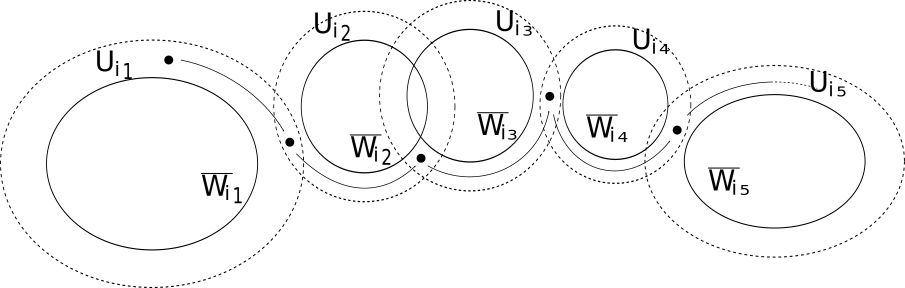
\includegraphics[scale=.5]{img/and-schori-bigger.pdf}
      \caption{Potencjalna wędrówka punktu $z$ generująca nieskończony łańcuch}
    \end{figure}
    
    Niech $z \in U_k$. Zauważmy, że do tego aby $g_n(z) \neq z$ potrzeba aby $pz \in U_n$. Przypuśćmy, że istnieje nieskończenie wiele $g_n$ ruszających kolejne obrazy $z$, tzn. ciąg $h_n(z)$ nie jest od pewnego pewnego momentu stały. Oznaczmy wszystkie funkcje powodujące zmiany przez $g_{i_1}, g_{i_2}, \dots$. Wówczas jednak $pz \in U_{i_1}$, a więc i $p g_{i_1}(z) \in U_{i_1}$. Dalej $p g_{i_1}(z) \in U_{i_2}$, więc $p g_{i_2}(g_{i_1}(z)) \in U_{i_2}$. Proces ten kontynuujemy otrzymując łańcuch $U_{i_1}, U_{i_2}, \dots$, co jest sprzeczne z porządkiem łańcuchowo skończonym.

    
    Otrzymujemy więc poprawną określoność $h$. Wykażemy teraz iniektywność $h$. Niech $x, y \in M$. Skoro jednak $h := \lim h_n$ się stabilizuje to istnieje $n$ takie, że $h(x) = h_n(x) = h_n(y) = h(y)$. Z iniektywności $h_n$ dostajemy $x = y$.
    
    Wiemy, że $(W_n)_{n\in\Ni}$ jest pokryciem $M$, a więc $\im h \subset M$. Pokażemy, że $\im h = M$. Niech $y\in M$. Weźmy $n$ takie, że $y\in W_n$. Z homeomorficzności $h_n$ dostajemy pewne $x$ takie, że $h_n(x) = y$. Ale z własności $g_m$ dla każdego $m > n$ mamy $g_m(h_n(x)) = h_n(x)$ a więc i $h(x) = \lim h_m(x) = \lim g_m(g_{m-1}(\dots h_n(x))) = h_n(x) = y$.
    
    Przyjrzyjmy się teraz odwzorowaniu odwrotnemu. Z powyższych rozważań widzimy, że $h^{-1}$ na $W_n$ jest równe $h_n^{-1}|_{W_n}$. Zatem $h^{-1}$ jest bijekcją i lokalnie wygląda jak homoemorfizm $h_n^{-1}|_{W_n}$ pomiędzy zbiorami otwartymi a więc i samo jest homeomorfizmem.
  \end{proof}
\end{thm} 